The following section aims to provide an in-depth overview of select components central to the translator's functionality and describe the reasoning behind them.

\subsection{System architecture and execution control flow}
% todo overview, add class diagrams and flow charts @Johannes
The decoding of the RISC--V assembly is relatively straight-forward, as we have a fixed instruction length of 32 bits.
Thus, the assembly is parsed in 4 byte blocks with the information being extracted in an intermediate instruction format holding the mnemonic, operands and immediates in uncompressed form.
This intermediate format can then be used by special per-mnemonic translation functions which, in the end, generate the x86--64 byte code using faenc~\cite{faenc}.

\begin{figure}[h]
	\begin{center}
		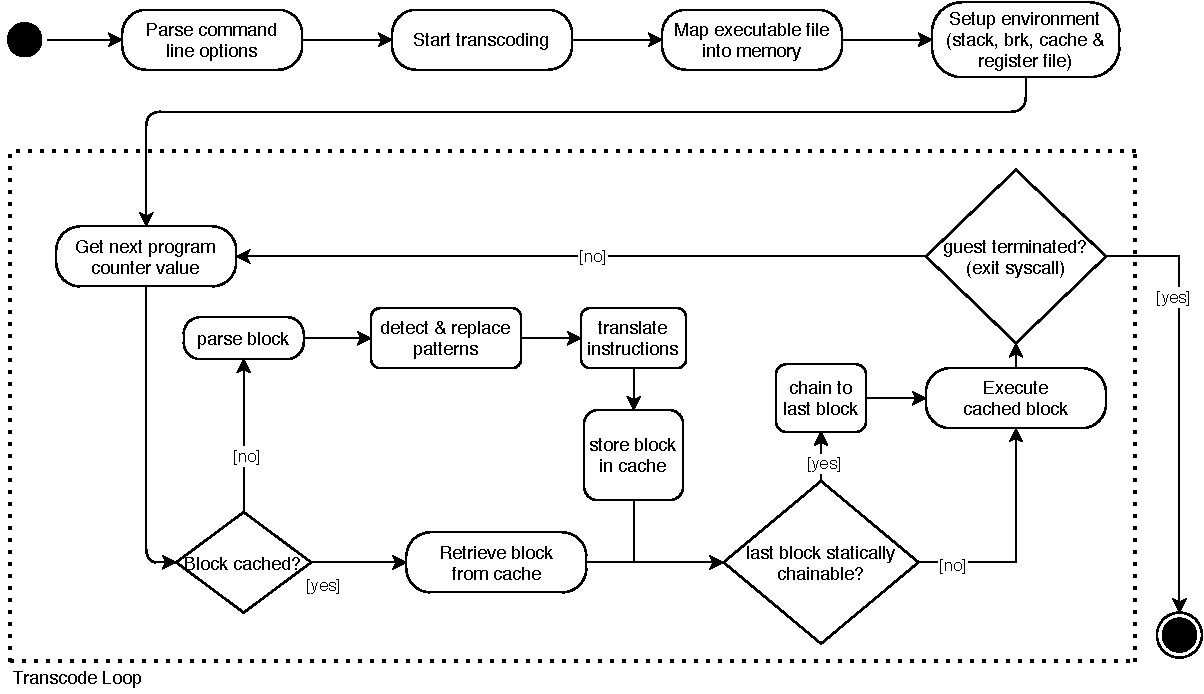
\includegraphics[width=\textwidth]{media/strategy.pdf}
		\caption{Control flow overview of the translation and execution process}
	\end{center}
\end{figure}



\subsection{Static hybrid register mapping}
\subsubsection{Register priority analysis}
In order to achieve the best performance with the hybrid approach to the register mapping described in section~\vref{sec:context-switch-reg-handle}, we must decide which registers of the RISC--V guest to map into the host's limited number of available GPRs.
There are two main ways of determining the priority of registers when considering them as candidates for a mapping.

It is, on the one hand, possible to assess the priority statically, by performing an analysis of the binary in question.
Essentially, the hereby produced metric counts the number of times the register is used in the assembly instructions listed in the guest program and thus delivers an idea of how important each register is to this specific executable.
We have built the tools required for this effort directly into the translator's analyser function, accessed via the \texttt{-a} flag.

However, this approach does not take into account that a single instruction may be executed many times while the program is running.
Accordingly, the other approach is to assess the register priority dynamically by analysing and profiling the execution of the testing program, thereby gaining an insight into how often each register is actually used during the execution.
The translator is also capable of performing such an analysis, commanded by the \texttt{-p} flag.
A dynamic analysis, of course, delivers a largely more accurate idea of the priority of the registers in question, but has the decided and obvious disadvantage that it cannot be performed without actually executing the binary.


\pgfplotstableread[col sep=comma,header=false]{benchmarks/register-frequency/freq.csv}\regfreqtable
\pgfplotstablesort[sort key =1, sort cmp=float >]\sortedregfreqtable{\regfreqtable}
\begin{figure}[h]
%\pgfplotstabletypeset\sortedregfreqtable
	\centering
	\makebox[\textwidth][c]{
	\begin{tikzpicture}
		\begin{axis}[%
			title = {Dynamic Register Usage Frequency},
			ybar,
			area legend,
			ylabel = {Access percentage},
			xtick = data,
			xticklabel style = {
				inner sep = 0pt,
				anchor = north east,
				rotate = 60,
				font=\footnotesize
			},
			ytick = {0.1, 0.2, 0.3, 0.4},
			scaled y ticks = false,
			x = 0.4cm,
			point meta = {y*100},
            nodes near coords = {\pgfmathprintnumber\pgfplotspointmeta\%},
			yticklabel = {\pgfmathparse{\tick*100}\pgfmathprintnumber{\pgfmathresult}\%},
			every node near coord/.append style = {font = \tiny, rotate = 90, anchor = west, /pgf/number format/fixed, /pgf/number format/precision = 2, color=black},
			enlarge x limits = {abs = 0.5cm},
			xtick={0,...,31},
			xticklabels from table = {\sortedregfreqtable}{0},
			ymin = 0, ymax = 0.45,
			ymajorgrids = true,
			bar width = 5pt,
			bar shift = 0,
			height = 7.0cm,
			width = \linewidth,
			legend style = {
				at = {(0.98, 0.97)},
				anchor = north east,
				legend columns = 3,
				column sep = 0.2cm
			}
		]
			\addplot+[fill=era-dbt-1, draw=black, restrict x to domain=0:12]table [x expr = \coordindex, y = 1]\sortedregfreqtable;
			\addplot+[fill=era-dbt-2, draw=black, restrict x to domain=13:31]table [x expr = \coordindex, y = 1]\sortedregfreqtable;

			\legend{statically mapped, not mapped}
		\end{axis}
	\end{tikzpicture}
	}
	\caption[Dynamic Register Usage Analysis]{The average results of a dynamic register usage analysis, ordered by frequency.}
	\label{fig:reg-usage}
\end{figure}


For the average results of such an analysis performed on a range of programs, including \textit{gzip}~\cite{gzip} and several benchmarks of the \texttt{intspeed}-Suite of \textit{SPEC CPU 2017}~\cite{spec-cpu-2017}, see figure~\ref{fig:reg-usage}.

Primarily, we gain interesting insights into the differences between the static and dynamic results yielded by the analysis.
While the static ranked hit list does not differ greatly between the different executables and the top $12$ entries are identical for every one of the tested programs, the dynamic results are far more variable.
This makes creating a register mapping that fits well to every executable very difficult.

The benchmarks \texttt{605.mcf} (route planning workload) and \texttt{620.omnetpp} (discrete event simulation for computer networking)~\cite{spec-cpu-doc} of the \textit{SPEC CPU} suite can serve as examples here.
For programs like \texttt{605.mcf} that only lightly use the stack, holding the stack pointer \texttt{sp/x2} in a native register when only $1,20\,\%$ of accesses actually utilise it would not be necessary.
However, other programs like \texttt{620.omnetpp} may rely heavily on the stack, and thus log very frequent accesses to \texttt{sp/x2};
when statistically every ninth access is to the stack pointer, it is absolutely essential to map the register to a native GPR\@.

If a static analysis yielded results of similar quality to the dynamic counterpart, the DBT could analyse the binary prior to execution and run every program with a best-fit static register mapping.
However, evidently, this is impossible with dynamic profiling.


\subsubsection{Structure of the mapping}
When we structure our mapping by the average case of the insights gained, we statistically capture about $83,59\,\%$ of register accesses, initially leaving the remaining $16,41\,\%$ to read from the register file in memory.
The following section will touch on our approach to optimise the accesses to the remaining not-statically-mapped registers.

From the 16 general-purpose registers x86--64 has to offer, we may use the 12 registers \texttt{rbx}, \texttt{rbp}, \texttt{rsi}, \texttt{rdi} and \texttt{r8}--\texttt{r15}.
The remaining registers have either implicit or exclusive functions in some instructions (\texttt{rax} and \texttt{rdx} for multiplication/division, \texttt{cl} for shifting), or, like \texttt{rsp}, are impractical to use in combination with block chaining and function calls.

Taking the 12 registers that are most accessed on average, the mapping structure is as seen in table~\vref{tab:static-register-mapping}.

\begin{table}
	\centering
	\makebox[\textwidth][c]{
	\begin{tabular}{rcccccccccccc}
		\toprule
		\textbf{RISC--V register} & \texttt{a5} & \texttt{a4} & \texttt{a3} & \texttt{a0} & \texttt{fp} & \texttt{sp} & \texttt{a2} & \texttt{a1} & \texttt{s1} & \texttt{ra} & \texttt{a7} & \texttt{s2}\\
		\textbf{x86--64 mapping} & \texttt{rbx} & \texttt{rbp} & \texttt{rsi} & \texttt{rdi} & \texttt{r8} & \texttt{r9} & \texttt{r10} & \texttt{r11} & \texttt{r12} & \texttt{r13} & \texttt{r14} & \texttt{r15}\\
		\bottomrule
	\end{tabular}
	}
	\caption[Active static register mapping]%
	{The static register mapping in use by the translator, ordered by the RISC--V register usage frequency (descending).}
	\label{tab:static-register-mapping}
\end{table}

\subsubsection{Dynamically allocated replacement registers}
\label{sec:lazy-replace-details}
In order to implement the desired temporary register replacement behaviour detailed in section~\ref{sec:context-switch-reg-handle}, we need to keep track of the age of the values currently situated in the replacement registers.
With that, we can implement a \textit{least recently used} register replacement policy.
To do this, we track a metric of \textit{replacement recency} (essentially serving as an inverse value age) for each block during translate-time.
This recency gets incremented for every access not captured by the static register mapping.

An access to a register that is not statically mapped then first checks the contents of all temporary registers -- if the value is already present, the DBT may use that value's register.
If it is not already present, the DBT selects any free replacement register if able, and otherwise selects the register with the oldest value (or minimal recency) for write-back.
The value is then loaded into the selected register from the register file in memory and marked as being the youngest in order to prevent it from being discarded in following mapping calls.

The dynamic mapping must also be able to receive requests for specific target registers for a load in order to support shifting and multiplication/division instructions that require arguments in implicitly defined registers.
In order to support this efficiently, the DBT is able to shuffle the values in the replacement registers around accordingly.

With this behaviour, we manage to greatly save on memory accesses to the register file compared to simply loading and storing the values on an instruction-by-instruction basis.
This style of register mapping can also not perform worse than accessing memory for each instruction, as in the worst case the DBT will perform the same memory accesses as with the other strategy, just possibly at a different time.

\begin{figure}[h]
\begin{subfigure}{0.45\textwidth}
\begin{lstlisting}[label={lst:without-lazy-replace}, showlines=true]




; add x6, x6, x7
mov	rax, [gp_file + 8 * 6]
mov	rdx, [gp_file + 8 * 7]
add	rax, rdx
mov	[gp_file + 8 * 6], rax

; slli x6, x6, 3
mov	rax, [gp_file + 8 * 6]
shl	rax, 3
mov	[gp_file + 8 * 6], rax

; xori x7, x7, -1
mov	rax, [gp_file + 8 * 7]
xor	rax, -1
mov	[gp_file + 8 * 7], rax




\end{lstlisting}
\subcaption{Without dynamic register mapping}
\end{subfigure}
\hfill
\begin{subfigure}{0.45\textwidth}
\begin{lstlisting}[label={lst:with-lazy-replace}, showlines=true]
; load registers
mov rdx, [gp_file + 8 * 6]
mov rcx, [gp_file + 8 * 7]

; add x6, x6, x7
add	rdx, rcx




; slli x6, x6, 3
shl	rdx, 3



; xori x7, x7, -1
xor	rcx, -1



; write back registers
mov [gp_file + 8 * 6], rdx
mov [gp_file + 8 * 7], rcx
\end{lstlisting}
\subcaption{With dynamic register mapping}
\end{subfigure}
\label{fig:lazy-replace-code}
\caption[Example assembly for dynamic register allocation]%
{A comparison of the code generated for example assembly by the DBT prior to and after introducing dynamic register allocation. The translated instructions are listed as a comment.}
\end{figure}



\subsection{Detailed system call overview}
As described in section~\vref{sec:syscall-handling}, we must assume the role of the kernel by handling system calls during the execution of the guest program.
We achieve this by translating the \texttt{ECALL} instruction as a context switch and jump to the \texttt{emulate\_ecall} routine in the DBT, which can then take the appropriate action.

As we stored the guest's registers before jumping to the handler, the requested system call index is now available to the DBT in the register file as entry \texttt{a7}, as per the RISC--V standard calling convention.
We may now handle the system calls based on that index and the arguments passed in the registers \texttt{a0} through \texttt{a6}, and write the return value to entry \texttt{a0} of the register file prior to switching the context back to the guest.

As previously mentioned, some system calls require special handling when encountered by the DBT (see table~\vref{tab:syscall-special} for details).
The following will describe the specifics of these issues with system calls that are either not present on the x86--64 host architecture, or may influence or break the state of the DBT\@.
\begin{description}
	\item[Adapting structure data format.]
	There are system calls like \texttt{fstat} and \texttt{fstatat} that exist both on RISC--V as well as x86--64, but use different data structure layouts in their return values.
	Thus, the DBT must adapt the host's returned data to the required format prior to passing it back to the guest.
	
	
	\item[Emulation required.]
	The DBT captures the \texttt{exit} and \texttt{exit\_group} calls.
	Passing them through would immediately terminate the DBT -- an action that is undesirable as it prevents any form of clean-up or post-execution profiling and analysis to take place.
	Thus, the DBT uses these system calls to set a flag which stops the translator's main loop from executing the next iteration.
	
	The \texttt{brk} system call must also be entirely emulated, as it would otherwise allow the guest program to modify the endpoint of the DBT's data segment (\textit{program break}), thus potentially deallocating some of the translator's memory.
	
	
	\item[Ignoring system calls.]
	The \texttt{rt\_sigaction} system call is ignored by the DBT\@.
	Due to the fact that the DBT and guest binary are running within the confines of the same process, any signal handler installed by the guest binary through \texttt{rt\_sigaction} would also capture the respective signal sent to the translator.
	As it is impossible to distinguish the DBT from the guest program in inter-process communication, we must ignore this call in order to avoid undefined behaviour on signal handling.
	
	
	\item[Guarded pass-through to host.]
	Essentially, any system call that has the possibility to influence the state or memory of the translator needs to have respective safe-guards in place.
	A good example of this behaviour is the \texttt{mmap} system call, the handling of which also reflects the memory layout scheme discussed in section~\vref{sec:memory-layout}.
	
	In any case, we must prevent a memory mapping into the translator's memory region.
	Mappings that do not interfere with the DBT's memory can be passed along to the host directly.
	In case a hinted mapping would conflict with the translator's memory, we may just re-hint the mapping to the top of the guest's address space.
	When the call is not hinted (the \texttt{MAP\_FIXED} or \texttt{MAP\_FIXED\_NOREPLACE} flag commands the mapping at exactly the specified address), we are unable to provide the guest with the requested mapping;
	thus we simulate an existing mapping in the location in question by returning \texttt{EEXIST} for \texttt{MAP\_FIXED\_NOREPLACE} and failing the call with \texttt{EINVAL} for \texttt{MAP\_FIXED}.
	
	Similarly, we fail the guest's \texttt{munmap} with \texttt{EINVAL} in cases where the translator's memory would be compromised by the de-allocation.
\end{description}

The other supported system calls may be directly passed through to the host after performing the necessary index mapping.
With this strategy, we are able to support the following system calls:
\begin{multicols}{4}
	\begin{itemize*}
		\item \texttt{getcwd}
		\item \texttt{fcntl}
		\item \texttt{ioctl}
		\item \texttt{unlinkat}
		\item \texttt{ftruncate}
		\item \texttt{faccessat}
		\item \texttt{chdir}
		\item \texttt{fchmod}
		\item \texttt{fchown}
		\item \texttt{pipe2}
		\item \texttt{openat}
		\item \texttt{close}
		\item \texttt{getdents64}
		\item \texttt{lseek}
		\item \texttt{read}
		\item \texttt{write}
		\item \texttt{writev}
		\item \texttt{readlinkat}
		\item \texttt{utimensat}
		\item \texttt{set\_tid\_address}
		\item \texttt{futex}
		\item \texttt{set\_robust\_list}
		\item \texttt{clock\_gettime}
		\item \texttt{tgkill}
		\item \texttt{rt\_sigprocmask}
		\item \texttt{uname}
		\item \texttt{gettimeofday}
		\item \texttt{getpid}
		\item \texttt{getuid}
		\item \texttt{geteuid}
		\item \texttt{getgid}
		\item \texttt{getegid}
		\item \texttt{gettid}
		\item \texttt{sysinfo}
		\item \texttt{execve}
		\item \texttt{wait4}
		\item \texttt{prlimit64}
		\item \texttt{renameat2}
		\item \texttt{getrandom}
	\end{itemize*}
\end{multicols}

\begin{table}
	\centering
	\begin{tabular}{ccc}
		\toprule
		\textbf{System Call (index)} & \textbf{Handling} & \textbf{x86--64 base (index)}\\
		\midrule
		\texttt{fstatat} (79) & data reformat & \texttt{newfstatat} (262)\\
		\texttt{fstat} (80) & data reformat & \texttt{fstat} (5)\\
		\texttt{exit} (93) & emulate & n/a\\
		\texttt{exit\_group} (94) & emulate & n/a\\
		\texttt{rt\_sigaction} (134) & ignore & n/a\\
		\texttt{brk} (214) & emulate & n/a\\
		\texttt{munmap} (215) & guarded pass-through & \texttt{munmap} (11)\\
		\texttt{mmap} (222) & guarded pass-through & \texttt{mmap} (9)\\
		\bottomrule
	\end{tabular}
	% state: aa55cef4816eb790df21f4742b7cf1f29685da49
	\caption[Specially handled system calls overview]%
	{An overview of the system calls we support that require special handling by the binary translator.}
	\label{tab:syscall-special}
\end{table}


